\begin{filecontents*}[overwrite]{sample.bib}
@article{yeo2000new,
  title={A new family of power transformations to improve normality or symmetry},
  author={Yeo, In-Kwon and Johnson, Richard A},
  journal={Biometrika},
  year={2000}
}

@inproceedings{chen2016xgboost,
  title={XGBoost: A scalable tree boosting system},
  author={Chen, Tianqi and Guestrin, Carlos},
  booktitle={Proceedings of KDD '16},
  year={2016}
}

@article{muggeo2003estimating,
  title={Estimating regression models with unknown break-points},
  author={Muggeo, Vito M R},
  journal={Statistics in Medicine},
  year={2003}
}

@article{hansen2000sample,
  title={Sample splitting and threshold estimation},
  author={Hansen, Bruce E},
  journal={Econometrica},
  year={2000}
}
\end{filecontents*}



\documentclass[12pt,a4paper]{article}

\usepackage[paper=a4paper,
            left=35mm,
            right=35mm,
            top=30mm,
            bottom=30mm]{geometry}

\usepackage[utf8]{inputenc}
\usepackage[T1]{fontenc}
\usepackage{lmodern}
\usepackage{microtype}
\usepackage{setspace}
\usepackage{parskip}     
\usepackage{graphicx}
\graphicspath{{images/}}
\usepackage{caption}
\usepackage{subcaption}
\usepackage{booktabs}
\usepackage{amsmath,amssymb}
\usepackage{hyperref}
\usepackage{float}
\usepackage{enumitem}
\setlist{nosep}

% Header / footer (simple)
\usepackage{fancyhdr}
\pagestyle{fancy}
\fancyhf{}           
% clear all header/footer fields
\renewcommand{\headrulewidth}{0pt}   % remove top line
\renewcommand{\footrulewidth}{0pt}   % no bottom line
\fancyfoot[C]{\thepage}         % page number in bottom center


% Section numbering depth
\setcounter{secnumdepth}{3}
\setcounter{tocdepth}{3}

% Typography tweaks (Darshan-like simple style)
\usepackage{setspace}
\onehalfspacing


% ---------------- Titlepage ----------------
\begin{document}

\begin{titlepage}
\centering

\vspace*{1.6cm}

{\Huge\bfseries PROJECT REPORT\par}
\vspace{0.2cm}
{\Large\bfseries NATURAL LANGUAGE PROCESSING \par}
\vspace{0.8cm}

\includegraphics[width=0.38\textwidth]{amberg.svg.png}
\vspace{1.2cm}

{\Large\bfseries PROJECT HEADING\par}

\vspace{1.0cm}

\vspace{1.2cm}

{\large Submitted by\par}
\vspace{0.2cm}
{\Large\bfseries Hemanthkumar Muthusamy Gunasekaran\par}

\vspace{0.8cm}

{\large Supervised by\par}
\vspace{0.2cm}
{\Large\bfseries Prof. Dr. Patrick Levi\par}

\vfill

{\large\bfseries Ostbayerische Technische Hochschule Amberg--Weiden\par}
\vspace{0.25cm}
{\small Department of Electrical Engineering, Media and Computer Science\par}

\vspace{0.3cm}

{\large \today\par}

\end{titlepage}


% No table of contents, no lists of figures/tables (per request)

% ---------------- Abstract ----------------
\begin{center}
\section*{Abstract}
\end{center}
\addcontentsline{toc}{section}{Abstract}
This work implements a machine learning pipeline using an optimized XGBoost regressor to predict targets on unseen dataset. Work Package 1 establishes a system through RankGauss feature normalization, Yeo-Johnson target transformation . Work Package 2 focused arriving at a mathematical solution that is physically fit for the proposed deployment environment.

% ---------------- Main sections (from Report draft.pdf) ----------------
\section{Work Package 1: Feature Engineering}
\addcontentsline{toc}{section}{Work Package 1: Feature Engineering on the Data Set}

\subsection{Introduction and Baseline Analysis}
 Initial visualization revealed that the raw features were highly skewed with extreme outliers, while others varied only within narrow ranges. A baseline XGBoost model \cite{chen2016xgboost} trained on these raw features demonstrated severe instability its performance dropped sharply under minor noise injection, indicating reliance on unstable patterns. To address this, several actions has beeen carried out in the following sections explained.

\subsection{Feature Preprocessing}
\subsubsection{RankGauss Feature Normalization}
To address the effects of heavy-tailed distributions and outliers, applied RankGauss normalization. Unlike standard scaling this non-linear quantile to normal mapping forces feature ranks into a standard normal distribution while preserving relative ordering while creating Gaussian-like marginals.

\begin{figure}[H]
  \centering
  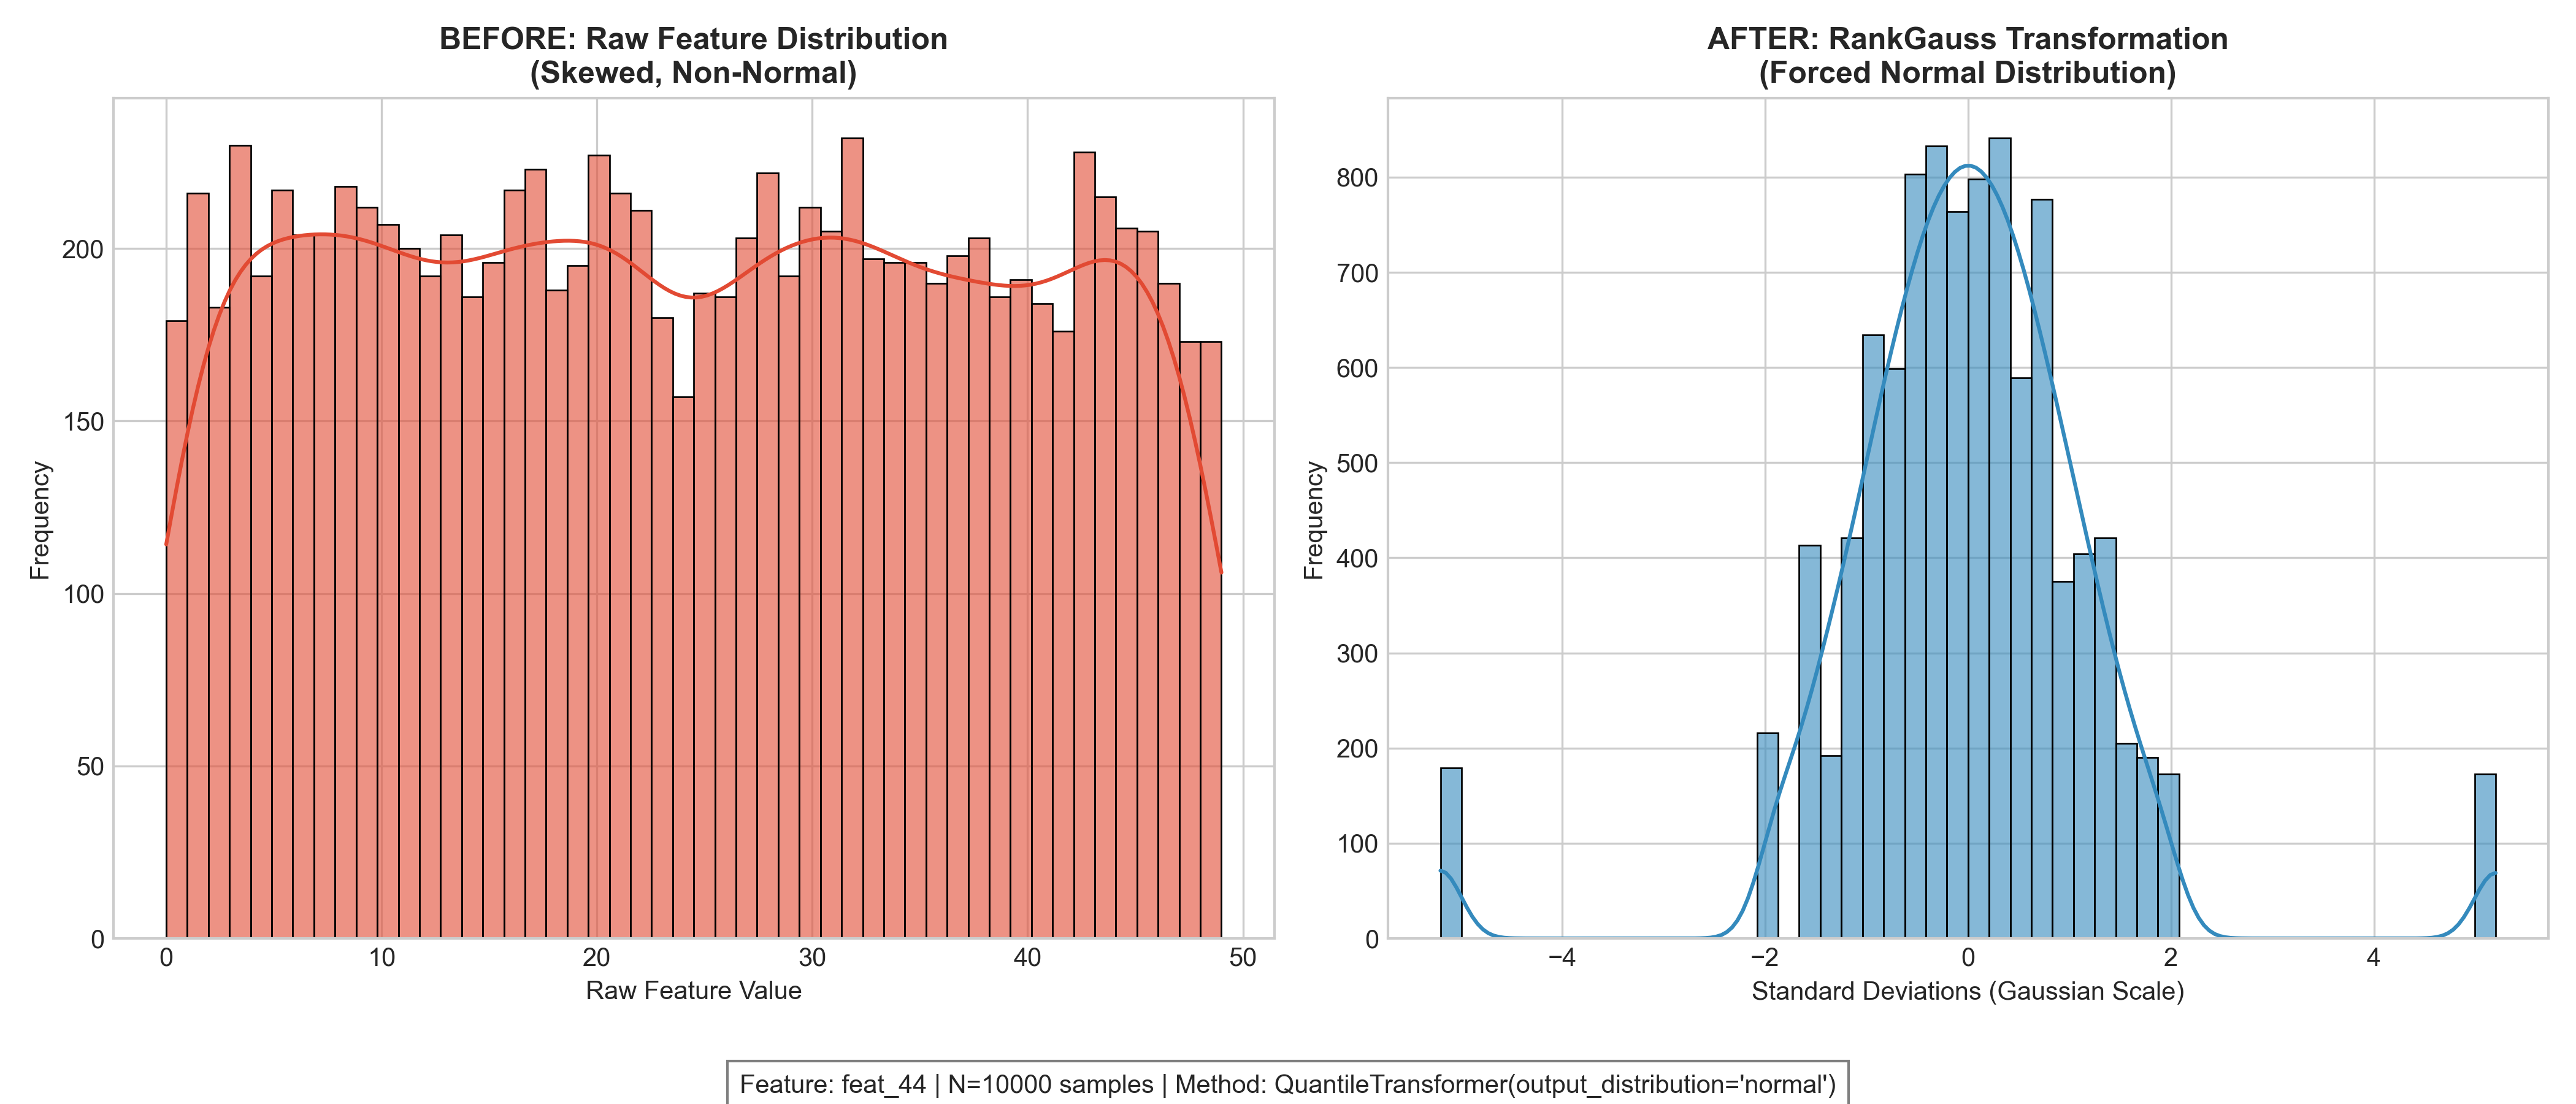
\includegraphics[width=0.9\linewidth]{05_rankgauss_transform_v2.png}
  \caption{Transformation of a representative feature from skewed raw input (left) to standard normal distribution (right) using RankGauss.}
  \label{fig:rankgauss}
\end{figure}

\subsubsection{Target Variable Stabilization}
The target variable exhibited significant skewness. A Yeo-Johnson Power Transformation \cite{yeo2000new} was applied to map the target to a symmetric. This ensures a symmetric error surface for faster convergence. Predictions are inverse transformed back to real units for final evaluation. The transformation $\psi(\lambda, y)$ is defined piecewise:

\begin{equation}
\psi(\lambda, y) =
\begin{cases}
\dfrac{(y+1)^{\lambda}-1}{\lambda}, & \text{if } y \ge 0 \text{ and } \lambda \ne 0,\\[8pt]
\ln(y+1), & \text{if } y \ge 0 \text{ and } \lambda = 0,\\[8pt]
-\dfrac{(-y+1)^{\,2-\lambda}-1}{2-\lambda}, & \text{if } y < 0 \text{ and } \lambda \ne 2,\\[8pt]
-\ln(-y+1), & \text{if } y < 0 \text{ and } \lambda = 2.
\end{cases}
\end{equation}

\subsubsection{Stabilized Feature Interactions}
A small set of interaction features were constructed to capture non-linear relations. Interactions were stabilized with functions such as \texttt{log1p} and \texttt{tanh} to prevent extreme values dominating the model which in trun enables learning of non-linear.

\subsection{Feature Selection}
\addcontentsline{toc}{subsection}{Feature Selection}

\subsubsection{Stability-Based Selection Method}
Feature selection was performed since features contained many unstable or redundant signals that encourage memorization. Selection used bootstrapped permutation importance measured across multiple splits; feature impact was summarized by mean importance and its variance across splits that were created.

\begin{figure}[H]
  \centering
  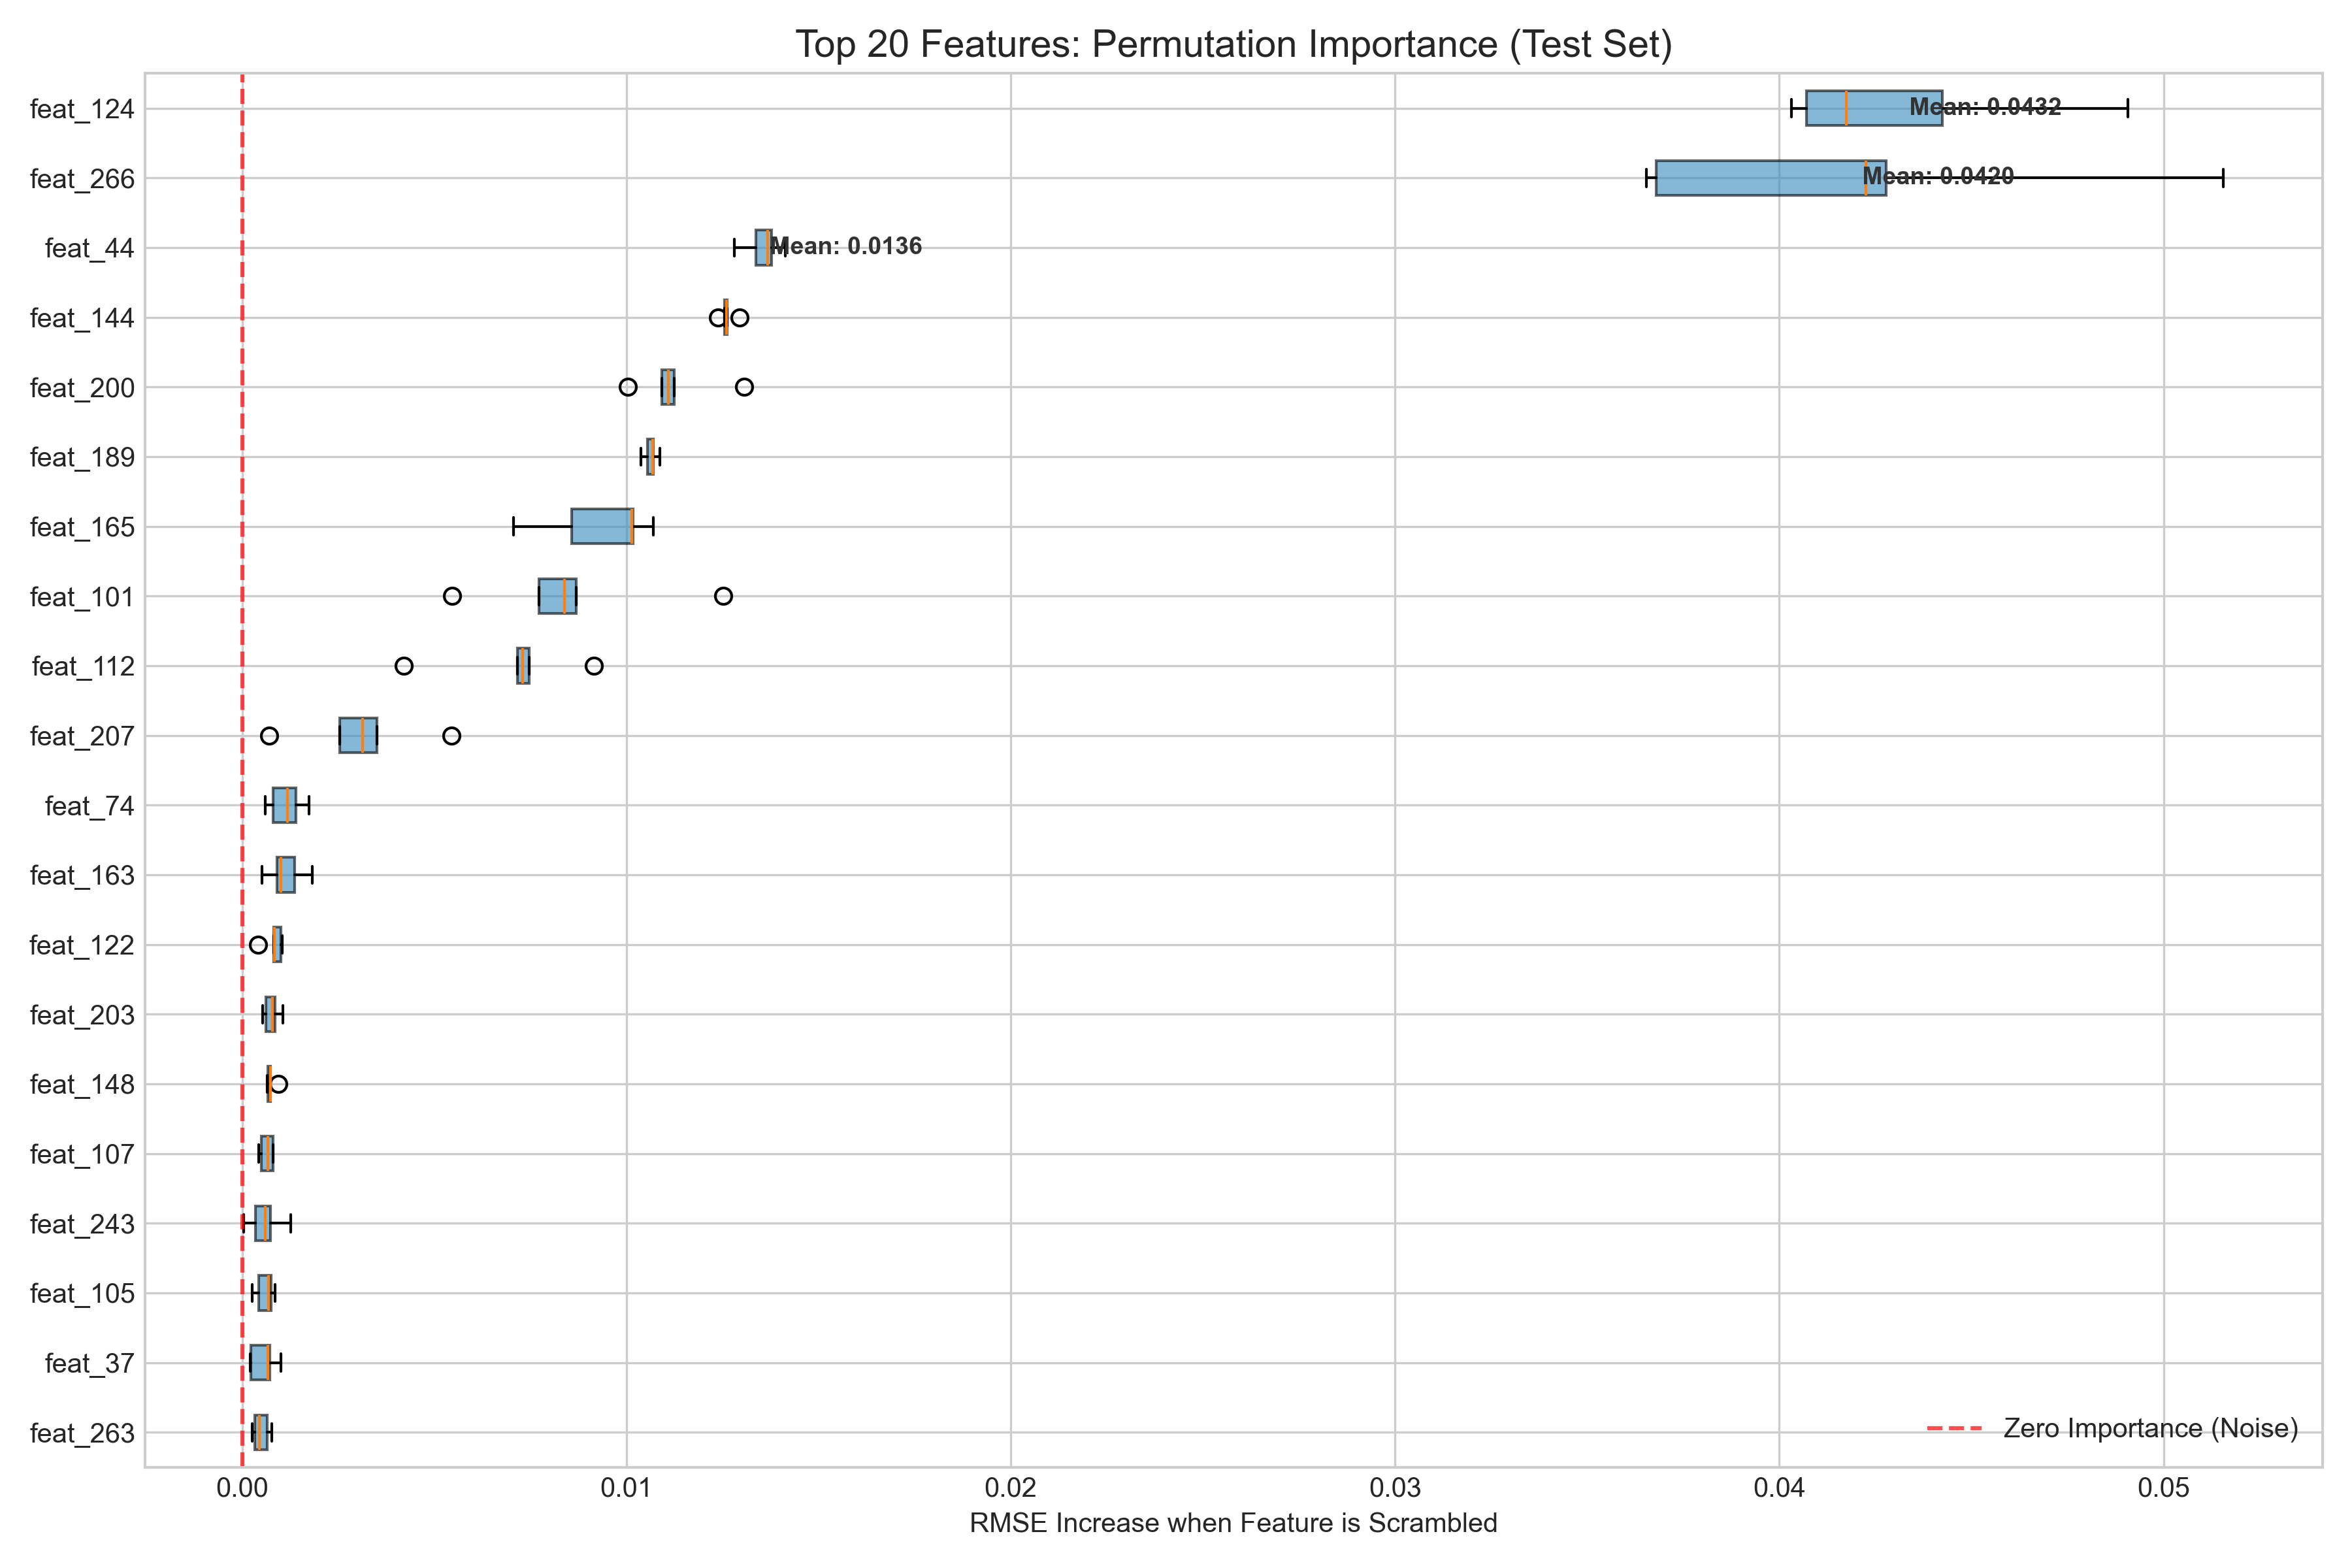
\includegraphics[width=0.5\linewidth]{01_permutation_importance_v2.png}
  \caption{Top features ranked by stability (permutation importance) across independent data splits, highlighting the inputs most critical for generalization.}
  \label{fig:feature_importance}
\end{figure}

\subsubsection{Construction of Feature Set}
Reducing the feature space was necessary to prevent complexity from overwhelming 
generalization. Features were ranked using a custom \textit{Stability Score} ($S_f$), 
defined as the ratio of a feature's mean permutation importance ($\mu_f$) to its 
volatility ($\sigma_f$) across the $K=5$ validation folds:

\begin{equation}
S_f \;=\; \frac{\mu_f}{\sigma_f + \varepsilon}
\end{equation}
where $\varepsilon$ is a small positive constant used to prevent division by zero.

\subsection{Model Training}
\addcontentsline{toc}{subsection}{Model Training}

\subsubsection{Model Training on Stable Features}
The XGBoost model was trained using only the stability-selected feature set and the transformed target variable. All preprocessing steps were fit exclusively on the training portion of each split and then applied unchanged to the corresponding validation data. This ensured that all reported generalization results are free form information leakage.

\subsubsection{Optuna-Based Optimization}
Hyperparameter optimization was performed using Optuna to identify a robust configuration for the selected feature set. Each trial was evaluated using a custom adversarial objective that penalized the baseline $R^2$ for performance degradation under 1\% relative feature noise and $0.5\sigma$ covariate shifts. This objective favored high-regularization configurations, including elevated L2 \texttt{reg\_lambda} and increased \texttt{min\_child\_weight}, in order to reduce sensitivity to distributional perturbations and improve out-of-distribution stability.

\subsubsection{Model Verification and Artifact saving}
Model selection and verification were performed using an 80/20 train--test split on the labeled dataset. On this split, the model achieved a training performance of $R^2 \approx 0.714$ and a held-out test performance of $R^2 \approx 0.501$. After hyperparameter optimization and feature selection were completed, the final model was retrained on the full 10{,}000-row labeled dataset in order to maximize the information available for deployment. The saved artifacts of the model were used to generate predictions for the unseen \texttt{EVAL\_29.csv} dataset. The file \texttt{EVAL\_target01\_29.csv} contains the corresponding predicted target values after applying all learned preprocessing steps and inverse target transformations.

\begin{figure}[H]
  \centering
  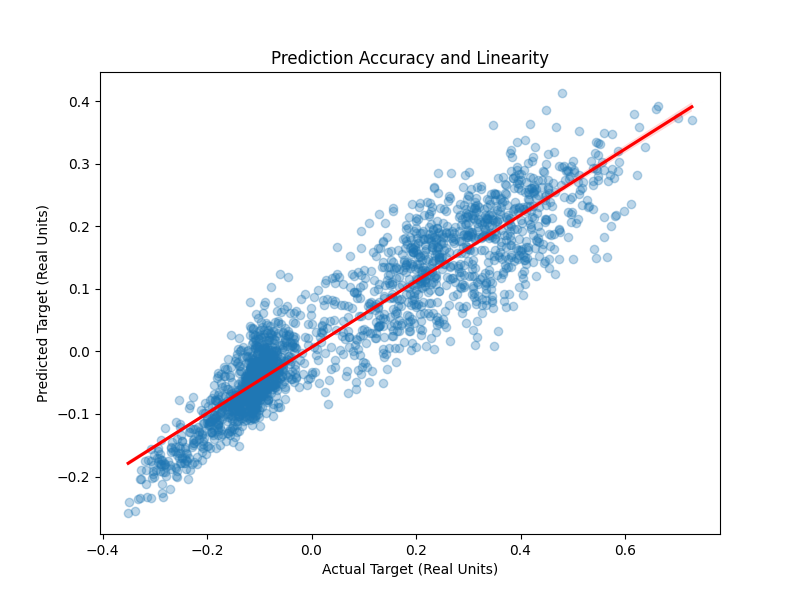
\includegraphics[width=0.6\linewidth]{final_prediction_accuracy.png}
  \caption{Predicted vs. Actual values }
  \label{fig:pred_vs_actual}
\end{figure}

\subsubsection{Robustness and Stability Tests}
Stability testing was conducted to quantify performance degradation in non-ideal scenarios. The system utilized a specialized \texttt{ModelAuditor} to measure $R^2$ sensitivity against 1\% relative noise injection, 0.5$\sigma$ covariate shifts, and K-Means error distribution across five data segments to identify potential blind spots.

\begin{table}[H]
\centering
\begin{tabular}{|l|c|}
\toprule
Metric & Mean value \\
\midrule
Baseline test $R^2$              & 0.501 \\
Noise test $R^2$ (1\% noise)     & 0.462 \\
Noise drop $\Delta R^2_{\text{noise}}$ & 0.039 \\
Drift test $R^2$ (0.5$\sigma$ shift) & 0.181 \\
Segmentation ratio              & 1.12 \\
\bottomrule
\end{tabular}
\caption{Robustness metrics computed on the held-out 20\% test set.}
\end{table}

\section{Work Package 2: Feature Engineering and Logic Derivation}
\addcontentsline{toc}{section}{Work Package 2: Feature Engineering and Logic Derivation}

\subsection{Introduction}
The primary objective of this task was to derive a prediction framework for \texttt{target02} suitable for deployment on an edge device with limited computational capacity. The problem was approached by two methods by starting with feature analysis and trying to find out the underlying pattern through a tree based regression model.

\subsection{Feature Preprocessing }

\subsubsection{Baseline Feature Analysis}
Initial correlation analysis was performed on all 273 input variables in \texttt{dataset\_29}. The plot in Figure~\ref{fig:feature_discovery}, \texttt{feat\_180} shows the dominant driver of \texttt{target02}, with a substantially higher correlation than any other feature. A second layer of influential variables is formed by \texttt{feat\_146} and \texttt{feat\_80}, followed by \texttt{feat\_200}. This distribution indicates that the target is controlled by a small number of strongly interacting signals rather than by a high-dimensional linear combination.

\begin{figure}[H]
\centering
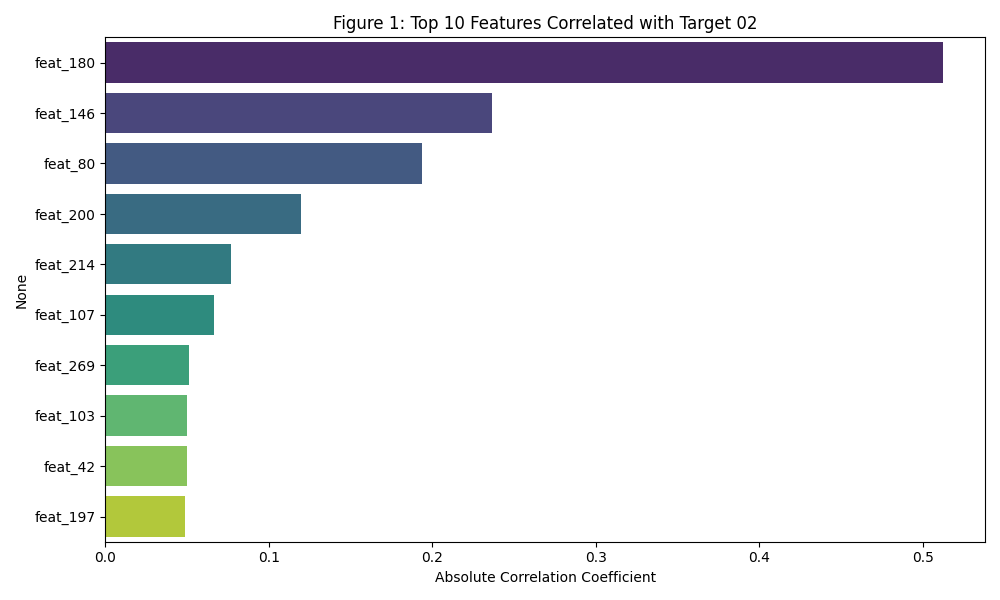
\includegraphics[width=0.85\textwidth]{Figure_1_Feature_Discovery.png}
\caption{Top correlated features with \texttt{target02}.}
\label{fig:feature_discovery}
\end{figure}

\subsubsection{Identifying the Underlying Mechanism}
The  \texttt{feat\_180} explains most of the variance, a single global regression produces large structured errors. Figure~\ref{fig:switch} reveals the reason: when plotting \texttt{target02} against \texttt{feat\_180} and coloring points by \texttt{feat\_80}, the data separates into multiple parallel linear bands. This demonstrates that \texttt{feat\_80} does not merely influence the magnitude of the target but selects between different linear regimes. Therefore, \texttt{feat\_80} functions as a discrete state variable that makes the system between multiple operating modes.

\begin{figure}[H]
\centering
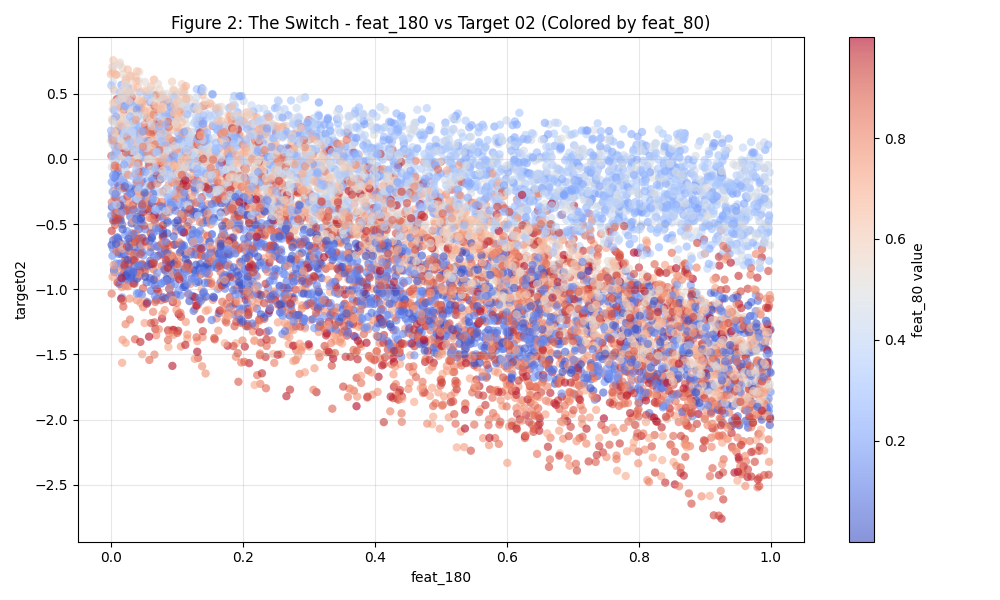
\includegraphics[width=0.85\textwidth]{Figure_2_The_Switch.png}
\caption{Switching behavior of \texttt{feat\_80} over the \texttt{feat\_180}–\texttt{target02} relationship.}
\label{fig:switch}
\end{figure}

\subsection{Feature Selection and the Ghost Variable}

\subsubsection{Residual Structure and Missing Physics}
After modeling the switching behavior of \texttt{feat\_80}, significant residual structure remained and were correlated against all unused features which  revealing a strong linear dependence on \texttt{feat\_200}, as shown in Figure~\ref{fig:ghost}. This indicates that \texttt{feat\_200} acts as a hidden correction term, adding or subtracting an offset that is invisible in the primary \texttt{feat\_180} projection. Together with \texttt{feat\_146}. The turning boundaries of \texttt{feat\_80} were found at 0.20, 0.50, and 0.70, defining four distinct operating zones.

\begin{figure}[H]
\centering
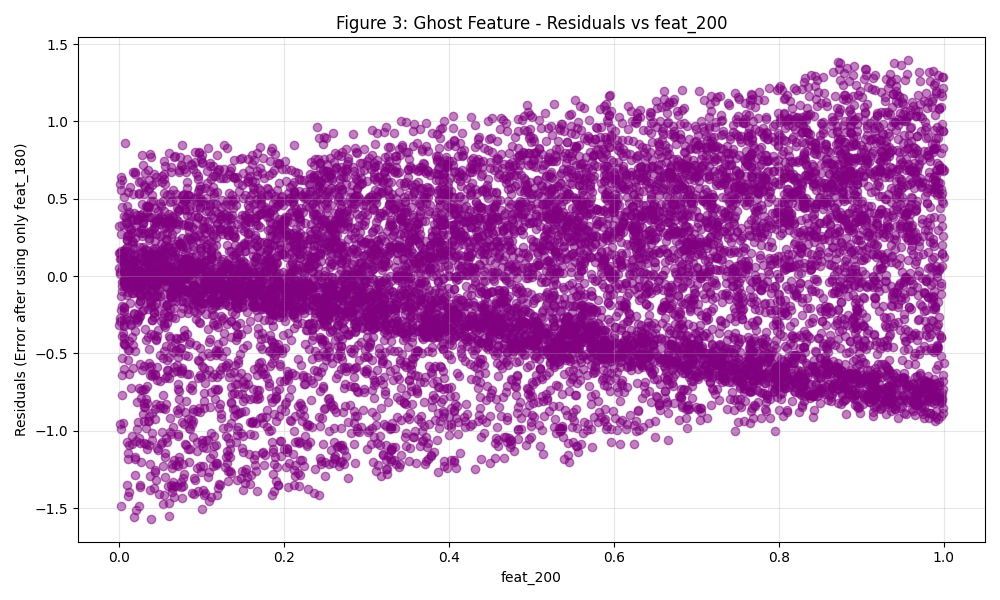
\includegraphics[width=0.85\textwidth]{Figure_3_Ghost_Feature.png}
\caption{Residuals from the \texttt{feat\_180}-only model as a function of \texttt{feat\_200}.}
\label{fig:ghost}
\end{figure}

\subsection{Model Training and Equation Derivation}

Ordinary Least Squares regression was applied independently within each of the four \texttt{feat\_80} zones, using \texttt{feat\_180}, \texttt{feat\_200}, and \texttt{feat\_146}. This produced four piecewise linear equations, \cite{muggeo2003estimating} each valid in a specific physical regime:

\begin{itemize}
\item \textbf{Zone 1:} \texttt{feat\_80} $\leq 0.20$
\item \textbf{Zone 2:} $0.20 < \texttt{feat\_80} \leq 0.50$
\item \textbf{Zone 3:} $0.50 < \texttt{feat\_80} \leq 0.70$
\item \textbf{Zone 4:} $\texttt{feat\_80} > 0.70$
\end{itemize}

The above mentioned structure provides the end reuslt which was the goal to attain.

\subsection{Hyperparameter Validation}

Thresholds at 0.20, 0.50, and 0.70 were validated by five-fold perturbation testing ($\pm0.02$ shifts increased RMSE to $\sim$0.21, $p<10^{-5}$) confirming true regime boundaries \cite{hansen2000sample}.

\subsection{Evaluation of findings }

\subsubsection{Accuracy Verification}
The final piecewise framework was implemented in \texttt{framework\_29.py} and evaluated on the full dataset and found that the model provides a stable and accurate piecewise linear approximation of the underlying relationships in the data.

% ---------------- References ----------------
\bibliographystyle{ieeetr} % or 'plain', 'apalike', etc.
\bibliography{sample}  % links to references.bib
\section*{Declaration of Generative AI Usage}
\addcontentsline{toc}{section}{Declaration of Generative AI Usage}

During the preparation of this work, generative AI tools (ChatGPT) were used for
\begin{itemize}
    \item improving grammar, clarity and writing quality
    \item assisting with code debugging and formatting.
\end{itemize}


\end{document}